% !TEX TS-program = xepythontex



\documentclass[10pt,envcountsect,spanish]{beamer}


\newif\ifnotas
\notasfalse% Para no mostrar los globos
\notastrue % Para  mostrar los globos

\input ../preambulo.tex



%································ TITULO, AUTOR, ETC
\title{Clases y Objetos}
\subtitle{Tecnología de la Programación}


\author[L. Daniel Hernández]{L. Daniel Hernández $<ldaniel@um.es>$}

\institute[ldaniel@um.es]{Dpto. Ingeniería de la Información  y las Comunicaciones\\ Universidad de Murcia\\\today\\\,\\\hrule} %	 \\ \today\\ \hrule}


\date[ldaniel@um.es]{ 
\vskip 1.25cm
%\vskip -1.25cm
%\includegraphics[width=.8\textwidth, height=.18\textheight]{fig/polinomio}
}

\graphicspath{{img/}}



%%%%%%%%%%%%%%%%%%%%%%%%%%%%%%%%%%
%%%%%%%%%%%%%%%%%%%%%%%%%%%%%%%%%%
%%%%%%%%%%%%%%%%%%%%%%%%%%%%%%%%%%
%%%%%%%%%%%%%%%%%%%%%%%%%%%%%%%%%%

%https://es.overleaf.com/learn/how-to/Writing_Markdown_in_LaTeX_Documents
\usepackage[hashEnumerators]{markdown}


%%%%%%%%%%%%%%%%%%%%%%%%%%%%%%%%%%
%%%%%%%%%%%%%%%%%%%%%%%%%%%%%%%%%%
%%%%%%%%%%%%%%%%%%%%%%%%%%%%%%%%%%
%%%%%%%%%%%%%%%%%%%%%%%%%%%%%%%%%%
\begin{document}

%\pgfdeclareimage[height=1cm]{logo}{logo.png}
%\logo{\pgfuseimage{logo}}



%--------------------------------------------------------------------------------
{\usebackgroundtemplate{%
  \includegraphics[width=\paperwidth,height=\paperheight]{../img/fondoUMUCompleto}}
\begin{frame}[b]
	\maketitle

\begin{tikzpicture}[overlay, remember picture]
\node[anchor=south west, %anchor is bottom left corner of the graphic
      xshift=.4\textwidth, %shifting around
      yshift=0.0cm] 
     at (current page.south west) %left bottom corner of the page
     {\includegraphics[width=.4\textwidth, height=.4\textheight]{fig/claseObjetos2}}; 
\end{tikzpicture}
	
\end{frame}			% Transparencia: Título
}



%--------------------------------------------------------------------------------
%%%%%%%%%%%%%%%%%%%%%%%%%%%%%%%%%%
%%%%%%%%%%%%%%%%%%%%%%%%%%%%%%%%%%
\begin{frame}{Índice de Contenidos}\tableofcontents \end{frame}




%%%%%%%%%%%%%%%%%%%%%%%%%%%%%%%%%%
%%%%%%%%%%%%%%%%%%%%%%%%%%%%%%%%%%
\section{Abstracción}




%%%%%%%%%%%%%%%%%%%%%%%%%%%%%%%%%%
%%%%%%%%%%%%%%%%%%%%%%%%%%%%%%%%%%
\subsection{Resumen}

% ===============================================================================================
% ===============================================================================================
\begin{frame}{Resumen sobre la abstracción}


\begin{itemize}
\item La \key{abstracción}  es el proceso mental por el que captamos las \key[red]{características principales} de un concepto o proceso descartando los detalles aíslando conceptualmente las distintas partes, propiedades o cualidades de un objeto para estudiarlas por separado. 

\item Genera grupos jerárquicos: cada grupo es una abstracción que ignora algunas características de los elementos que forman parte de él. 


\item Mecanismos de abstracción:
\begin{itemize} 

\item \key{Parametrización}. Se usan parámetros para representar a un conjunto de elementos.

\item \key{Especificación}. Cumplimentar documentos indicando nombre, descripción y condiciones.

\end{itemize}


\item {Tipos de Abstracción}: procedimental, iteración y abstracción de datos.

\item Hay 3 niveles de abstracción de datos: tipos de datos integrados, tipos de datos definidos por el usuario, Tipos de Datos Abstractos.
\end{itemize}


\end{frame}
%% . . . . . . . . . . . . . . . . . . . . . . . . . . . . . . . . . . . . . . . . . . . . . . . . . . . . . . 
%% . . . . . . . . . . . . . . . . . . . . . . . . . . . . . . . . . . . . . . . . . . . . . . . . . . . . . . 





% ===============================================================================================
% ===============================================================================================
\begin{frame}{Resumen sobre los TDAs}
\begin{itemize}
\item  Los \key{Tipos de Datos Abstractos} (TDA) son \textbf{modelos matemáticos} que constan de

\begin{itemize}
\item un nombre publico para 
\item identificar a un conjunto de datos (valores), junto con
\item un conjunto de operaciones bien definidas sobre los datos (como en una estructura algebraica). 
\end{itemize}

\item Como modelo, le es \key{irrelevante} cómo se almacenan o estructuren los datos y cómo se implementan las operaciones.

\item Para todo TDA hemos de abordar \key{tres tareas}: 

\begin{itemize}
\item \textbf{Especificación:} definición del TDA 

\begin{itemize}
\item La \key{especificación} de un TDA (Datos+Operaciones) se rige por las normas generales de la \textit{\bf Abstracción por Especificación}

\item Se debe dar la especificación de los datos y de los operadores (constructores, modificadores y de consulta).

\item Hay que distinguir los operadores: fundamentales vs no fundamentales, públicos vs privados.
\end{itemize}


\item \textbf{Representación:} estructura con la que representar el TDA. Debe definir:

\begin{itemize}
\item \key{La función de abstracción.} Una función sobreyectiva $Abst: \mbox{\textbf{rep}} \longrightarrow {\cal A}$ 

\item \key{El invariante de la representación.} Es un predicado
$I: \mbox{\textbf{rep}} \longrightarrow \mathbb{B}$ que es cierto para los objetos de \textbf{rep} que sean legítimos.
\end{itemize}

\item \textbf{Implementación:} cómo implementar la estructura en un lenguaje de programación.

\end{itemize}

\end{itemize}
\end{frame}
%% . . . . . . . . . . . . . . . . . . . . . . . . . . . . . . . . . . . . . . . . . . . . . . . . . . . . . . 
%% . . . . . . . . . . . . . . . . . . . . . . . . . . . . . . . . . . . . . . . . . . . . . . . . . . . . . . 







%%%%%%%%%%%%%%%%%%%%%%%%%%%%%%%%%%
%%%%%%%%%%%%%%%%%%%%%%%%%%%%%%%%%%
\section{Programación Orientada a Objetos}



%%%%%%%%%%%%%%%%%%%%%%%%%%%%%%%%%%
%%%%%%%%%%%%%%%%%%%%%%%%%%%%%%%%%%
\subsection{Principios de la POO}

% ===============================================================================================
% ===============================================================================================
\begin{frame}{Principios de la POO}

\begin{itemize}
\item \small \key[red]{Nuestro Objetivo:} 

\centerline{\bf \underline{Usar} la POO para \underline{implementar} TDAs (que son modelos matemáticos) \underline{en} \cm[red]{Python}.}

\item Conceptos asociados a la POO

\begin{itemize} 
\item \key{Abstracción} es un proceso mental de extracción de las características esenciales de un concepto o proceso descartando los detalles. Hay dos tipos de abstracción:

\begin{itemize}
\item TDA: Abstracción de tipo
\item POO: Abstracción operacional
\end{itemize}


\item \key{Encapsulamiento.} Proceso por el que se agrupan datos y operaciones, ocultando los detalles internos.

\begin{itemize}
\item No se oculta la información, sino su soporte. 
\item La información se accede por una interface.
\end{itemize}


\item \key{Jerararquización}. Estructurar por niveles (jerarquía) los elementos que intervienen en el proceso.

\begin{itemize}
\item Jerarquía de clasificación (\textbf{Herencia}).

\item Jerarquía de composición (\textbf{Asociación, agregación})
\end{itemize}



\item \key{Modularidad}. Descomposicón del sistema en conjunto de módulos poco acoplados (independientes) y cohesivos (con significado propio)
\end{itemize}

\end{itemize}


\end{frame}
%% . . . . . . . . . . . . . . . . . . . . . . . . . . . . . . . . . . . . . . . . . . . . . . . . . . . . . . 
%% . . . . . . . . . . . . . . . . . . . . . . . . . . . . . . . . . . . . . . . . . . . . . . . . . . . . . . 







%%%%%%%%%%%%%%%%%%%%%%%%%%%%%%%%%%
%%%%%%%%%%%%%%%%%%%%%%%%%%%%%%%%%%
\subsection{Clases}


%%%%%%%%%%%%%%%%%%%%%%%%%%%%%%%%%%%%%
%%%%%%%%%%%%%%%%%%%%%%%%%%%%%%%%%%%%%
\begin{frame}{ TDA $\color{white} \Rightarrow $ Clase. Clase $\color{white} \not \Rightarrow$ TDA} 


\begin{itemize}
\item Diseñar un TDA es \key{abstraer} lo que tienen de común entes parecidos: calculadoras, estudiantes, coches,  ...

\

\centerline{\includegraphics[width=.25\textwidth]{fig/calweb}
\includegraphics[width=.25\textwidth, height=.25\textheight]{fig/estudiantes}
\includegraphics[width=.25\textwidth, height=.25\textheight]{fig/audis}
}

\item \unEjemplo Consideremos \key{dos estudiantes}. Ambos parecen tener \textbf{coincidencias} en
\begin{itemize}
\item Los mismos atributos: están en un curso, tienen una edad, ...
\item Los mismos comportamientos: se desplazan, estudian, cambian objetos en la mochila, ...
\end{itemize}

Realmente dos estudiantes se \key{diferencian}  en los valores de algunos atributos pero tienen los \key{mismos comportamientos/métodos} (con resultados posiblemente \textbf{diferentes} dependiendo de sus atributos).

\item Cuando \textbf{un conjunto de objetos presentan los mismos métodos y se diferencian solo en los estados}, diremos que dicho conjunto es una \key{clase} en POO.

\hfil \key{TDA} es el término formal. \key{Clase} es el término en POO. Pero no son lo mismo.

\item \key[red]{Los TDAs y las clases son tipos de datos.}
\end{itemize}
\end{frame}
% . . . . . . . . . . . . . . . . . . . . . . . . . . . . . . . . . . . . . . . . . . . . . . . . . . . . . . 
% . . . . . . . . . . . . . . . . . . . . . . . . . . . . . . . . . . . . . . . . . . . . . . . . . . . . . . 




%%%%%%%%%%%%%%%%%%%%%%%%%%%%%%%%%%%%%
%%%%%%%%%%%%%%%%%%%%%%%%%%%%%%%%%%%%%
\begin{frame}[fragile]{Declaración de clases} 


\begin{itemize}
\item Un \key{clase} es el término usado en programación para implementar un TDA en POO.

\item Informalmente, \key{una clase es una plantilla}/molde para construir los objetos.

\item En \cm[red]{Pseudocódigo}, una primera aproximación es el siguiente esquema:

{\small
\begin{code}[]%[basicstyle=\ttfamily\tiny]
class Car:
    # Variables posibles para definir un objeto
    luces: bool  # booleano on/off
    color: str   # string
    # 
    # Métodos
    None turnHeadLights():
        luces = not luces
    None moveForward():
        ...
\end{code}
}


\begin{enumerate}
\item Se usa la palabra reservada \cm[red]{class}
\item Se da un nombre a la clase \texttt{Car} (conjunto de objetos)
\item Se indican los atributos comunes de todos los objetos: variables
\item Se indican los métodos comunes de todos los objetos: similar a las funciones.
\end{enumerate}
\end{itemize}
\end{frame}
% . . . . . . . . . . . . . . . . . . . . . . . . . . . . . . . . . . . . . . . . . . . . . . . . . . . . . . 
% . . . . . . . . . . . . . . . . . . . . . . . . . . . . . . . . . . . . . . . . . . . . . . . . . . . . . . 




%%%%%%%%%%%%%%%%%%%%%%%%%%%%%%%%%%%%%
%%%%%%%%%%%%%%%%%%%%%%%%%%%%%%%%%%%%%
\begin{frame}{Ejercicio} 

\begin{example}

Desarrolla una aproximación inicial para declarar las clases correspondientes a los siguientes tipos de objetos:
\begin{enumerate}
\item funciones matemáticas,
\item conjuntos,
\item estadística descriptiva básica.
\end{enumerate}
\end{example}

\end{frame}
% . . . . . . . . . . . . . . . . . . . . . . . . . . . . . . . . . . . . . . . . . . . . . . . . . . . . . . 
% . . . . . . . . . . . . . . . . . . . . . . . . . . . . . . . . . . . . . . . . . . . . . . . . . . . . . . 




%%%%%%%%%%%%%%%%%%%%%%%%%%%%%%%%%%%%%
%%%%%%%%%%%%%%%%%%%%%%%%%%%%%%%%%%%%%
\begin{frame}{Representación UML de una clase}

\centerline{\includegraphics[width=1.05\textwidth]{fig/claseUML}}
%%%%% Generado con  http://www.plantuml.com/  Copiar y pegar el siguiente enlace.
% http://www.plantuml.com/plantuml/png/ZPA_ZXCn4CPxFyLNRYH09A6A1Bg2AwWEyQVYA2Rh2MV9dbdiMQHJb8UvyWeAMjfzCPnLTdKAGQAoy_q-ZtvPpLKnojQdwDf8fU1jdz8zzWwxmD4lJ-TgWo26rtXv2jROPoP_8_7-u93OxjGlcyLqNJKBZ4-cODtK7pD-rVoWg7c3CJmu9seCqmwwEnbiS1qXchQPuHcHSFJZKpNopkQk-oneANMAhkVQfOuojuoYKTtxCGhYGqiP766XK_TEsjWNHQi2Yj-6tuBHg1P36oYwJvIsONYKQUJmYtp8nsulX3gAMkCy_2nMvwAoDgZKTomUeZPvRjLCqsowgQPfU3JrbrnlvQ8iQkJ95DzxHcRJB9I7XrkvFkFrZ5hG7MbYorfg1-79N-NvarxgVWo8X5tFOWmk-A29v1cApj9bTE1YmuCWf2vogcMgu8LpJnVefblEErJSuOoji9yseJIBl_3QkV66vr_kWlSiNz_y1rhz6otT5OllK_m3
%%%%%



\begin{ejercicio}{}
Haz la representación UML de la clase \cm{Car} de la transparencia anterior.
\end{ejercicio}


\end{frame}
% . . . . . . . . . . . . . . . . . . . . . . . . . . . . . . . . . . . . . . . . . . . . . . . . . . . . . . 
% . . . . . . . . . . . . . . . . . . . . . . . . . . . . . . . . . . . . . . . . . . . . . . . . . . . . . . 






%%%%%%%%%%%%%%%%%%%%%%%%%%%%%%%%%%%%%
%%%%%%%%%%%%%%%  SECTION   %%%%%%%%%%%%%%%
%%%%%%%%%%%%%%%%%%%%%%%%%%%%%%%%%%%%%
\subsection{Objetos. Encapsulamiento}




%%%%%%%%%%%%%%%%%%%%%%%%%%%%%%%%%%%%%
%%%%%%%%%%%%%%%%%%%%%%%%%%%%%%%%%%%%%
\begin{frame}{Encapsulamiento} 

\begin{itemize}
\item En POO \key[red]{una clase} es una plantilla y \key{define} un tipo de dato.
\item En POO \key[red]{un objeto} representa a una entidad (física o abstracta) que viene dado por la \key{particularización de una abstracción} (definida por una clase/TDA).

\item Un objeto presenta:
\begin{itemize}
\item Un \key[red]{estado}, dado por los valores concretos de sus \key{variables} de la representación.

Las variables también se llaman \key{atributos} o \key{campos}.

\item Un \key[red]{comportamiento}, representado por los \key{métodos} (realmente atributos precedimentales).
\end{itemize}

\item Estas dos componentes, juntas (o agrupadas) definen al objeto. 

\item La agrupación se llama \key{encapsulamiento}:

\end{itemize}

\centerline{\includegraphics[width=.5\textwidth]{fig/capsula}}
\vskip -0.5cm
\centerline{ \tiny Fuente \href{https://www.lineaysalud.com/que-es/capsulas-de-gelatina}{www.lineaysalud.com}}

\begin{itemize}
\item El \key{encapsulamiento} es el proceso por el que \textbf{un objeto} tiene sus propios datos y métodos.

\item La encapsulamiento requiere que su atributos queden \key{ocultos} (pero se estudiará con más detenimiento con los modificadores de acceso)

\end{itemize}
\end{frame}
% . . . . . . . . . . . . . . . . . . . . . . . . . . . . . . . . . . . . . . . . . . . . . . . . . . . . . . 
% . . . . . . . . . . . . . . . . . . . . . . . . . . . . . . . . . . . . . . . . . . . . . . . . . . . . . . 

















%%%%%%%%%%%%%%%%%%%%%%%%%%%%%%%%%%%%%
%%%%%%%%%%%%%%%  SECTION   %%%%%%%%%%%%%%%
%%%%%%%%%%%%%%%%%%%%%%%%%%%%%%%%%%%%%
\subsection{Constructores de Objetos}

%%%%%%%%%%%%%%%%%%%%%%%%%%%%%%%%%%%%%
%%%%%%%%%%%%%%%%%%%%%%%%%%%%%%%%%%%%%
\begin{frame}[fragile]{Constructores de Objetos}


\begin{itemize}
\item Para trabajar con clases y objetos:
	\begin{itemize}
	\item Hay que \key{indicar antes} cuál es  \textbf{la clase}.
	\item y \key{después} \textbf{los objetos} que la componen indicando cuál es el estado de cada uno.
	\end{itemize}

\item Para construir objetos, se necesitan \key{constructores}.

\item Un \key[red]{constructor} es un método especial que se caracteriza porque:
	\begin{itemize}
	\item No retorna nunca un valor
	\item Se llama igual que la clase
	\item Sus parámetros se identifican con algunos atributos.
	\item[] Por tanto, sus argumentos establecen el estado inicial del objeto.
	\end{itemize}

\item La construcción genera \key{una referencia} al objeto (ver ciclo de vida).

\item Algunos ejemplos para la clase \cm[blue]{Car} en \cm[red]{pseudocódigo} son:

{\footnotesize
\begin{code}[]%[basicstyle=\ttfamily\tiny]
  Car()                    {luces = false;  color="rojo";}
  Car(String c)            {luces = false;  color=c;}
  Car(boolean l)           {luces = l;  color="blanco";}
  Car(boolean l, String c) {luces = l;  color=c;}
\end{code}
}


\item Para construir un objeto, en \cm[red]{pseudocódigo}:

{\small
\begin{code}[basicstyle=\ttfamily\footnotesize]
c1 = Car();            // Luces apagadas, color rojo
c2 = Car("green");     // Luces apagadas, color verde
c3 = Car(true);        // Luces encendidas, color blanco
c4 = Car(true, "blue");// Luces encendidas, color azul
\end{code}
}


\end{itemize}
\end{frame}
% . . . . . . . . . . . . . . . . . . . . . . . . . . . . . . . . . . . . . . . . . . . . . . . . . . . . . . 
% . . . . . . . . . . . . . . . . . . . . . . . . . . . . . . . . . . . . . . . . . . . . . . . . . . . . . . 






%%%%%%%%%%%%%%%%%%%%%%%%%%%%%%%%%%%%%
%%%%%%%%%%%%%%%%%%%%%%%%%%%%%%%%%%%%%
\begin{frame}[fragile]{Cambiando el Estado de un Objeto} 

\begin{itemize}
\item Se necesita una referencia, \cm{nombreObjeto}, para acceder a un objeto.

\item Para usar un atributo o  un método de un objeto se usa la \key{notación punto}.

	\begin{itemize}
	\item \cm{nombreObjeto}\cm[blue]{.atributo} \qquad referencia a un atributo del objeto.
	\item \cm{nombreObjeto}\cm[blue]{.metodo()} \qquad referencia a un método del objeto.
	\end{itemize}
	
	
\item[] \unEjemplo 
{\small 
\begin{pyverbatim}[][frame=single]
c1.lights         # Referencia a la variable lights del coche c1
c2.moveForward()  # Referencia al método del coche c2.
\end{pyverbatim}
}

\item \key{Modificar el estado} de un objeto es cambiar los valores de sus variables/atributos.
\begin{itemize}
\item \key{No se deben modificar} los valores de los atributos \key{directamente.}\\
\hfil \textbf{Los motivos se explicarán en el siguiente tema.}
	
\item \key{La modificación del estado de un objeto se debe de realizar mediante sus métodos}

\item[] \unEjemplo \textsf{Acceso a un método para cambiar el estado}

\begin{pyverbatim}[][frame=single]
car.turnHeadLightsTo(true) # Cambia el estado de la luz
car.ligths = true          # Esto funciona pero está mal
\end{pyverbatim}

\end{itemize}
\end{itemize}
\end{frame}
% . . . . . . . . . . . . . . . . . . . . . . . . . . . . . . . . . . . . . . . . . . . . . . . . . . . . . . 
% . . . . . . . . . . . . . . . . . . . . . . . . . . . . . . . . . . . . . . . . . . . . . . . . . . . . . . 





%%%%%%%%%%%%%%%%%%%%%%%%%%%%%%%%%%%%%
%%%%%%%%%%%%%%%%%%%%%%%%%%%%%%%%%%%%%
\begin{frame}[fragile=singleslide]{El objeto \cm[yellow]{self}}

\begin{itemize}
\item En POO se suele usar un objeto especial (\cm{this}, \cm{self} o \cm{Me}) 
\item \fbox{\cm{self} se refiere al \key{objeto} que actualmente está ejecutando el código}.

\begin{itemize}
\item Recuerda que \cm{obj}\cm[blue]{.atributo} y \cm{obj}\cm[blue]{.metodo()} hace referencia al atributo \cm[blue]{.atributo} y al método \cm[blue]{.metodo()} del objeto \cm{obj}.

\item Por tanto,  \cm{self}\cm[blue]{.atributo} y \cm{self}\cm[blue]{.metodo()} hace referencia al atributo \cm[blue]{.atributo} y al método \cm[blue]{.metodo()} \textbf{del objeto que esté ejecutando el código} en ese momento.
\end{itemize}


\item \unEjemplo Considera el siguiente código \cm[red]{Python}

{\footnotesize\tt
\begin{pyverbatim}[][frame=single, numbers=left]
class Estudiante:
   ...
   def notaPOO (self, nota):
       self.nota = nota  # self.variable = parámetro

maria = Estudiante()
maria.notaPOO(10)
\end{pyverbatim}
}



\begin{itemize}[nosep] \footnotesize
\item \texttt{maria} es el objeto que ejecuta el código (línea 7).
\item \texttt{maria}\texttt{\color{blue}.notaPOO({\color{gray}10})}   hace referencia  al método \texttt{\color{blue} notaPOO()} para el objeto \texttt{maria}.
\item En la ejecución,  se realizará la instrucción \cm{self}\texttt{.nota = 10} (línea 4)
\item Como el objeto que lo invoca es \texttt{maria},  el objeto \cm{self} es el objeto \; \texttt{maria} (línea 4)

Es como si ejecutáramos:  \texttt{maria.nota = 10} 
\item En consecuencia, \textit{al objeto \cm{maria} se le asignará un 10 a su atributo} \cm{nota}.
\end{itemize}
\end{itemize}
\end{frame}
% . . . . . . . . . . . . . . . . . . . . . . . . . . . . . . . . . . . . . . . . . . . . . . . . . . . . . . 
% . . . . . . . . . . . . . . . . . . . . . . . . . . . . . . . . . . . . . . . . . . . . . . . . . . . . . . 






%%%%%%%%%%%%%%%%%%%%%%%%%%%%%%%%%%%%%
%%%%%%%%%%%%%%%%%%%%%%%%%%%%%%%%%%%%%
\begin{frame}[fragile]{Ciclo de vida de un objeto} 

\vskip -0.35cm
\begin{columns}[t]
\begin{column}{.67\textwidth}
\begin{itemize}
\item Es distinto un objeto que una referencia a un objeto.
\item El objeto está en el \key{Heap} y la referencia en \key[red]{Stack}.
\item Para que un objeto exista, éste necesita una referencia.
\item Para la \key{creación} se necesita

	\begin{itemize}
	\item Hacer una \textbf{declaración} del ``objeto''\/,
	%%\tikz[remember picture, overlay]\node (objeto){}; 
	indicando a qué clase pertenece - \textsf{opcional, según Lenguaje}.
	
	\item \textbf{Construir} un objeto, invocando al constructor de objetos.
	\item \textbf{Almacenar} la referencia retornada por el constructor.
	%\item \textbf{Asignar} una referencia al ``objeto'' creándolo.%\!\!\tikz[remember picture, overlay]\node (new){};
	%\\ El objeto lo construye un constructo
	\end{itemize}
Cada objeto se llama también \key{instancia de clase}.
\item Mientras que exista se puede \key{modificar} su estado.\!\! \tikz[remember picture, overlay]\node (mod){};
	
	\begin{itemize}
	\item El estado se modifica siempre \textbf{a través de los métodos}
	\end{itemize}


\item Un objeto \key{deja de existir} si no tiene una referencia a él. %\!\! \tikz[remember picture, overlay]\node (del){};

\begin{itemize}
\item El \key{recolector de basura} lo borrará de la memoria.
\item No es lo mismo \cm{car=None} que \cm{del(car)}
\end{itemize}
\end{itemize}


\textbf{No haremos  distinción entre objeto y referencia de objeto} \small (se entenderá por el contexto)

\end{column}

\begin{column}{.28\textwidth}

\begin{code}[numbers=none]
// Si procede
Car car;
  
car = Car(); 
\end{code}


\tikzset{every picture/.style={line width=0.75pt}} %set default line width to 0.75pt        

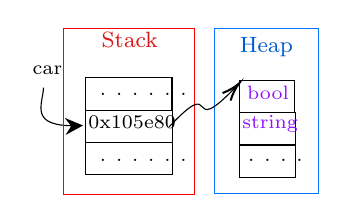
\begin{tikzpicture}[x=0.75pt,y=0.75pt,yscale=-1,xscale=1, scale=.8]
%uncomment if require: \path (0,300); %set diagram left start at 0, and has height of 300

%Shape: Rectangle [id:dp9235973719267798] 
\draw   (109.13,227) -- (161.33,227) -- (161.33,246.5) -- (109.13,246.5) -- cycle ;
%Shape: Rectangle [id:dp943958814863431] 
\draw   (109.13,246.5) -- (161.33,246.5) -- (161.33,266) -- (109.13,266) -- cycle ;
%Curve Lines [id:da17130432046514787] 
\draw    (83.63,213.5) .. controls (83.14,223.93) and (74.42,237.18) .. (104.47,236.37) ;
\draw [shift={(107.38,236.25)}, rotate = 537.01] [fill={rgb, 255:red, 0; green, 0; blue, 0 }  ][line width=0.08]  [draw opacity=0] (10.72,-5.15) -- (0,0) -- (10.72,5.15) -- (7.12,0) -- cycle    ;
%Shape: Rectangle [id:dp5830246329949738] 
\draw   (109.13,207.5) -- (161,207.5) -- (161,227) -- (109.13,227) -- cycle ;
%Shape: Rectangle [id:dp48074139763543533] 
\draw   (201.79,228.5) -- (235.17,228.5) -- (235.17,248) -- (201.79,248) -- cycle ;
%Shape: Rectangle [id:dp41398164171161844] 
\draw   (201.79,248) -- (235.17,248) -- (235.17,267.5) -- (201.79,267.5) -- cycle ;
%Shape: Rectangle [id:dp269043366445451] 
\draw   (201.79,209) -- (234.92,209) -- (234.92,228.5) -- (201.79,228.5) -- cycle ;
%Shape: Rectangle [id:dp33139522631185603] 
\draw  [color={rgb, 255:red, 0; green, 117; blue, 255 }  ,draw opacity=1 ] (186.67,178) -- (249.33,178) -- (249.33,277.33) -- (186.67,277.33) -- cycle ;
%Shape: Rectangle [id:dp3591489776533294] 
\draw  [color={rgb, 255:red, 253; green, 0; blue, 0 }  ,draw opacity=1 ] (95.67,177.67) -- (174.33,177.67) -- (174.33,278) -- (95.67,278) -- cycle ;
%Curve Lines [id:da3115856474476093] 
\draw    (159.33,237) .. controls (191.01,203.34) and (167.15,247.11) .. (200.31,212.09) ;
\draw [shift={(201.33,211)}, rotate = 493.14] [color={rgb, 255:red, 0; green, 0; blue, 0 }  ][line width=0.75]    (10.93,-3.29) .. controls (6.95,-1.4) and (3.31,-0.3) .. (0,0) .. controls (3.31,0.3) and (6.95,1.4) .. (10.93,3.29)   ;

% Text Node
\draw (109,229) node [anchor=north west][inner sep=0.75pt]  [font=\scriptsize] [align=left] {0x105e80};
% Text Node
\draw (75.5,199) node [anchor=north west][inner sep=0.75pt]  [font=\scriptsize] [align=left] {car};
% Text Node
\draw (116,255) node [anchor=north west][inner sep=0.75pt]  [font=\scriptsize] [align=left] {. . . . . .};
% Text Node
\draw (116,215) node [anchor=north west][inner sep=0.75pt]  [font=\scriptsize] [align=left] {. . . . . .};
% Text Node
\draw (201.79,228.5) node [anchor=north west][inner sep=0.75pt]  [font=\scriptsize] [align=left] {\textcolor[rgb]{0.56,0.07,1}{string}};
% Text Node
\draw (205.29,255) node [anchor=north west][inner sep=0.75pt]  [font=\scriptsize] [align=left] {. . . .};
% Text Node
\draw (204.67,211) node [anchor=north west][inner sep=0.75pt]  [font=\scriptsize] [align=left] {\textcolor[rgb]{0.56,0.07,1}{bool}};
% Text Node
\draw (200.33,181.33) node [anchor=north west][inner sep=0.75pt]  [font=\footnotesize,color={rgb, 255:red, 0; green, 92; blue, 204 }  ,opacity=1 ] [align=left] {Heap};
% Text Node
\draw (117,178.33) node [anchor=north west][inner sep=0.75pt]  [font=\footnotesize,color={rgb, 255:red, 216; green, 21; blue, 21 }  ,opacity=1 ] [align=left] {Stack};
\end{tikzpicture}%\tikz[remember picture, overlay]\node (modCod){};

\begin{code}[numbers=none]
car.turnHeadLights();

car = None;
\end{code}

%\hfil \tikz[remember picture, overlay]\node (delCod){};
 
\tikzset{every picture/.style={line width=0.75pt}} %set default line width to 0.75pt        

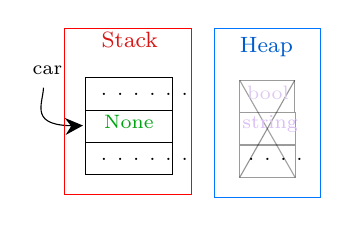
\begin{tikzpicture}[x=0.75pt,y=0.75pt,yscale=-1,xscale=1, scale=0.8]
%uncomment if require: \path (0,300); %set diagram left start at 0, and has height of 300

%Shape: Rectangle [id:dp9926817141242739] 
\draw   (108.46,94.67) -- (160.67,94.67) -- (160.67,114.17) -- (108.46,114.17) -- cycle ;
%Shape: Rectangle [id:dp13474023090439013] 
\draw   (108.46,114.17) -- (160.67,114.17) -- (160.67,133.67) -- (108.46,133.67) -- cycle ;
%Curve Lines [id:da6321855175932614] 
\draw    (82.96,81.17) .. controls (82.47,91.59) and (73.76,104.84) .. (103.81,104.03) ;
\draw [shift={(106.71,103.92)}, rotate = 537.01] [fill={rgb, 255:red, 0; green, 0; blue, 0 }  ][line width=0.08]  [draw opacity=0] (10.72,-5.15) -- (0,0) -- (10.72,5.15) -- (7.12,0) -- cycle    ;
%Shape: Rectangle [id:dp04501158379774406] 
\draw   (108.46,75.17) -- (160.5,75.17) -- (160.5,94.67) -- (108.46,94.67) -- cycle ;
%Shape: Rectangle [id:dp4801901358857874] 
\draw  [color={rgb, 255:red, 155; green, 155; blue, 155 }  ,draw opacity=1 ] (201.13,96.17) -- (234.5,96.17) -- (234.5,115.67) -- (201.13,115.67) -- cycle ;
%Shape: Rectangle [id:dp1675879518192791] 
\draw  [color={rgb, 255:red, 155; green, 155; blue, 155 }  ,draw opacity=1 ] (201.13,115.67) -- (234.5,115.67) -- (234.5,135.17) -- (201.13,135.17) -- cycle ;
%Shape: Rectangle [id:dp7635778334676109] 
\draw  [color={rgb, 255:red, 155; green, 155; blue, 155 }  ,draw opacity=1 ] (201.13,76.67) -- (234.25,76.67) -- (234.25,96.17) -- (201.13,96.17) -- cycle ;
%Shape: Rectangle [id:dp313073840798459] 
\draw  [color={rgb, 255:red, 0; green, 117; blue, 255 }  ,draw opacity=1 ] (186,45.67) -- (250,45.67) -- (250,147.33) -- (186,147.33) -- cycle ;
%Shape: Rectangle [id:dp8905054855352863] 
\draw  [color={rgb, 255:red, 253; green, 0; blue, 0 }  ,draw opacity=1 ] (95.67,45.33) -- (172.33,45.33) -- (172.33,145.67) -- (95.67,145.67) -- cycle ;
%Straight Lines [id:da6777714441381015] 
\draw [color={rgb, 255:red, 0; green, 0; blue, 0 }  ,draw opacity=0.37 ]   (201.13,76.67) -- (234.5,135.17) ;
%Straight Lines [id:da963608608807669] 
\draw [color={rgb, 255:red, 0; green, 0; blue, 0 }  ,draw opacity=0.42 ]   (234.25,76.67) -- (201.13,135.17) ;

% Text Node
\draw (74.83,66.67) node [anchor=north west][inner sep=0.75pt]  [font=\scriptsize] [align=left] {car};
% Text Node
\draw (116,122) node [anchor=north west][inner sep=0.75pt]  [font=\scriptsize] [align=left] {. . . . . .};
% Text Node
\draw (116,83) node [anchor=north west][inner sep=0.75pt]  [font=\scriptsize] [align=left] {. . . . . .};
% Text Node
\draw (201.13,96.17) node [anchor=north west][inner sep=0.75pt]  [font=\scriptsize,color={rgb, 255:red, 208; green, 2; blue, 27 }  ,opacity=1 ] [align=left] {\textcolor[rgb]{0.86,0.75,0.96}{string}};
% Text Node
\draw (204.63,122) node [anchor=north west][inner sep=0.75pt]  [font=\scriptsize] [align=left] {. . . .};
% Text Node
\draw (204,78.67) node [anchor=north west][inner sep=0.75pt]  [font=\scriptsize,color={rgb, 255:red, 74; green, 144; blue, 226 }  ,opacity=1 ] [align=left] {\textcolor[rgb]{0.87,0.79,0.95}{bool}};
% Text Node
\draw (199.67,49) node [anchor=north west][inner sep=0.75pt]  [font=\footnotesize,color={rgb, 255:red, 0; green, 92; blue, 204 }  ,opacity=1 ] [align=left] {Heap};
% Text Node
\draw (116.33,46) node [anchor=north west][inner sep=0.75pt]  [font=\footnotesize,color={rgb, 255:red, 216; green, 21; blue, 21 }  ,opacity=1 ] [align=left] {Stack};
% Text Node
\draw (117.92,96.42) node [anchor=north west][inner sep=0.75pt]  [font=\scriptsize,color={rgb, 255:red, 0; green, 163; blue, 16 }  ,opacity=1 ] [align=left] {None};


\end{tikzpicture}

\end{column}
\end{columns}



%
%\begin{tikzpicture}[remember picture, overlay]
%\draw[-, color=blue] (objeto) -- (objetoCod);
%\draw[-, color=blue] (new) -- (newCod);
%\draw[-, color=blue] (mod) -- (modCod);
%\draw[-, color=blue] (del) -- (delCod);
%\end{tikzpicture}
\end{frame}
% . . . . . . . . . . . . . . . . . . . . . . . . . . . . . . . . . . . . . . . . . . . . . . . . . . . . . . 
% . . . . . . . . . . . . . . . . . . . . . . . . . . . . . . . . . . . . . . . . . . . . . . . . . . . . . . 




%%%%%%%%%%%%%%%%%%%%%%%%%%%%%%%%%%%%%
%%%%%%%%%%%%%%%  SECTION   %%%%%%%%%%%%%%%
%%%%%%%%%%%%%%%%%%%%%%%%%%%%%%%%%%%%%
\subsection{POO para Resolver Problemas}





% ===============================================================================================
% ===============================================================================================
\begin{frame}{Cómo se usa la POO para Resolver Problemas}



\begin{columns}
\begin{column}{.6\textwidth}
\begin{itemize}
\item En todo problema se pueden identificar \key{conceptos}.
\item Cada concepto definirá una \key{clase} (define antes un TDA).

\begin{itemize}
\item Define un plantilla: \\ estructura (datos) + métodos (operaciones)
\end{itemize}


\item En un problema se identificarán entes/\key{objetos} concretos.

\begin{itemize}
\item Un objeto se crea con un estado inicial.
\item \key{Estado:} valores de sus atributos/estructura.
\end{itemize}

\end{itemize}
\end{column}

\begin{column}{.3\textwidth}


\tikzset{every picture/.style={line width=0.75pt}} %set default line width to 0.75pt        

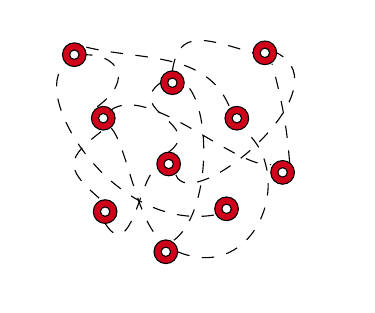
\begin{tikzpicture}[x=0.75pt,y=0.75pt,yscale=-1,xscale=1, scale = 0.45]
%uncomment if require: \path (0,400); %set diagram left start at 0, and has height of 400

%Shape: Donut [id:dp1930178134206031] 
\draw  [fill={rgb, 255:red, 208; green, 2; blue, 27 }  ,fill opacity=1 ,even odd rule] (124.6,60.67) .. controls (124.6,57.87) and (126.87,55.6) .. (129.67,55.6) .. controls (132.46,55.6) and (134.73,57.87) .. (134.73,60.67) .. controls (134.73,63.46) and (132.46,65.73) .. (129.67,65.73) .. controls (126.87,65.73) and (124.6,63.46) .. (124.6,60.67)(117,60.67) .. controls (117,53.67) and (122.67,48) .. (129.67,48) .. controls (136.66,48) and (142.33,53.67) .. (142.33,60.67) .. controls (142.33,67.66) and (136.66,73.33) .. (129.67,73.33) .. controls (122.67,73.33) and (117,67.66) .. (117,60.67) ;
%Shape: Donut [id:dp2135243958053359] 
\draw  [fill={rgb, 255:red, 208; green, 2; blue, 27 }  ,fill opacity=1 ,even odd rule] (193.6,98.67) .. controls (193.6,95.87) and (195.87,93.6) .. (198.67,93.6) .. controls (201.46,93.6) and (203.73,95.87) .. (203.73,98.67) .. controls (203.73,101.46) and (201.46,103.73) .. (198.67,103.73) .. controls (195.87,103.73) and (193.6,101.46) .. (193.6,98.67)(186,98.67) .. controls (186,91.67) and (191.67,86) .. (198.67,86) .. controls (205.66,86) and (211.33,91.67) .. (211.33,98.67) .. controls (211.33,105.66) and (205.66,111.33) .. (198.67,111.33) .. controls (191.67,111.33) and (186,105.66) .. (186,98.67) ;
%Shape: Donut [id:dp6542308498253413] 
\draw  [fill={rgb, 255:red, 208; green, 2; blue, 27 }  ,fill opacity=1 ,even odd rule] (50.6,98.67) .. controls (50.6,95.87) and (52.87,93.6) .. (55.67,93.6) .. controls (58.46,93.6) and (60.73,95.87) .. (60.73,98.67) .. controls (60.73,101.46) and (58.46,103.73) .. (55.67,103.73) .. controls (52.87,103.73) and (50.6,101.46) .. (50.6,98.67)(43,98.67) .. controls (43,91.67) and (48.67,86) .. (55.67,86) .. controls (62.66,86) and (68.33,91.67) .. (68.33,98.67) .. controls (68.33,105.66) and (62.66,111.33) .. (55.67,111.33) .. controls (48.67,111.33) and (43,105.66) .. (43,98.67) ;
%Shape: Donut [id:dp8870389277935447] 
\draw  [fill={rgb, 255:red, 208; green, 2; blue, 27 }  ,fill opacity=1 ,even odd rule] (120.6,147.67) .. controls (120.6,144.87) and (122.87,142.6) .. (125.67,142.6) .. controls (128.46,142.6) and (130.73,144.87) .. (130.73,147.67) .. controls (130.73,150.46) and (128.46,152.73) .. (125.67,152.73) .. controls (122.87,152.73) and (120.6,150.46) .. (120.6,147.67)(113,147.67) .. controls (113,140.67) and (118.67,135) .. (125.67,135) .. controls (132.66,135) and (138.33,140.67) .. (138.33,147.67) .. controls (138.33,154.66) and (132.66,160.33) .. (125.67,160.33) .. controls (118.67,160.33) and (113,154.66) .. (113,147.67) ;
%Shape: Donut [id:dp5224010308184139] 
\draw  [fill={rgb, 255:red, 208; green, 2; blue, 27 }  ,fill opacity=1 ,even odd rule] (242.6,156.67) .. controls (242.6,153.87) and (244.87,151.6) .. (247.67,151.6) .. controls (250.46,151.6) and (252.73,153.87) .. (252.73,156.67) .. controls (252.73,159.46) and (250.46,161.73) .. (247.67,161.73) .. controls (244.87,161.73) and (242.6,159.46) .. (242.6,156.67)(235,156.67) .. controls (235,149.67) and (240.67,144) .. (247.67,144) .. controls (254.66,144) and (260.33,149.67) .. (260.33,156.67) .. controls (260.33,163.66) and (254.66,169.33) .. (247.67,169.33) .. controls (240.67,169.33) and (235,163.66) .. (235,156.67) ;
%Shape: Donut [id:dp6814528997743807] 
\draw  [fill={rgb, 255:red, 208; green, 2; blue, 27 }  ,fill opacity=1 ,even odd rule] (52.6,198.67) .. controls (52.6,195.87) and (54.87,193.6) .. (57.67,193.6) .. controls (60.46,193.6) and (62.73,195.87) .. (62.73,198.67) .. controls (62.73,201.46) and (60.46,203.73) .. (57.67,203.73) .. controls (54.87,203.73) and (52.6,201.46) .. (52.6,198.67)(45,198.67) .. controls (45,191.67) and (50.67,186) .. (57.67,186) .. controls (64.66,186) and (70.33,191.67) .. (70.33,198.67) .. controls (70.33,205.66) and (64.66,211.33) .. (57.67,211.33) .. controls (50.67,211.33) and (45,205.66) .. (45,198.67) ;
%Shape: Donut [id:dp8701107499242482] 
\draw  [fill={rgb, 255:red, 208; green, 2; blue, 27 }  ,fill opacity=1 ,even odd rule] (223.6,28.67) .. controls (223.6,25.87) and (225.87,23.6) .. (228.67,23.6) .. controls (231.46,23.6) and (233.73,25.87) .. (233.73,28.67) .. controls (233.73,31.46) and (231.46,33.73) .. (228.67,33.73) .. controls (225.87,33.73) and (223.6,31.46) .. (223.6,28.67)(216,28.67) .. controls (216,21.67) and (221.67,16) .. (228.67,16) .. controls (235.66,16) and (241.33,21.67) .. (241.33,28.67) .. controls (241.33,35.66) and (235.66,41.33) .. (228.67,41.33) .. controls (221.67,41.33) and (216,35.66) .. (216,28.67) ;
%Shape: Donut [id:dp24447274944359032] 
\draw  [fill={rgb, 255:red, 208; green, 2; blue, 27 }  ,fill opacity=1 ,even odd rule] (19.6,30.67) .. controls (19.6,27.87) and (21.87,25.6) .. (24.67,25.6) .. controls (27.46,25.6) and (29.73,27.87) .. (29.73,30.67) .. controls (29.73,33.46) and (27.46,35.73) .. (24.67,35.73) .. controls (21.87,35.73) and (19.6,33.46) .. (19.6,30.67)(12,30.67) .. controls (12,23.67) and (17.67,18) .. (24.67,18) .. controls (31.66,18) and (37.33,23.67) .. (37.33,30.67) .. controls (37.33,37.66) and (31.66,43.33) .. (24.67,43.33) .. controls (17.67,43.33) and (12,37.66) .. (12,30.67) ;
%Shape: Donut [id:dp9012085358437154] 
\draw  [fill={rgb, 255:red, 208; green, 2; blue, 27 }  ,fill opacity=1 ,even odd rule] (182.6,195.67) .. controls (182.6,192.87) and (184.87,190.6) .. (187.67,190.6) .. controls (190.46,190.6) and (192.73,192.87) .. (192.73,195.67) .. controls (192.73,198.46) and (190.46,200.73) .. (187.67,200.73) .. controls (184.87,200.73) and (182.6,198.46) .. (182.6,195.67)(175,195.67) .. controls (175,188.67) and (180.67,183) .. (187.67,183) .. controls (194.66,183) and (200.33,188.67) .. (200.33,195.67) .. controls (200.33,202.66) and (194.66,208.33) .. (187.67,208.33) .. controls (180.67,208.33) and (175,202.66) .. (175,195.67) ;
%Shape: Donut [id:dp798249525379092] 
\draw  [fill={rgb, 255:red, 208; green, 2; blue, 27 }  ,fill opacity=1 ,even odd rule] (117.6,241.67) .. controls (117.6,238.87) and (119.87,236.6) .. (122.67,236.6) .. controls (125.46,236.6) and (127.73,238.87) .. (127.73,241.67) .. controls (127.73,244.46) and (125.46,246.73) .. (122.67,246.73) .. controls (119.87,246.73) and (117.6,244.46) .. (117.6,241.67)(110,241.67) .. controls (110,234.67) and (115.67,229) .. (122.67,229) .. controls (129.66,229) and (135.33,234.67) .. (135.33,241.67) .. controls (135.33,248.66) and (129.66,254.33) .. (122.67,254.33) .. controls (115.67,254.33) and (110,248.66) .. (110,241.67) ;
%Curve Lines [id:da3754267456514244] 
\draw  [dash pattern={on 4.5pt off 4.5pt}]  (49.33,86.33) .. controls (89.33,56.33) and (70.33,31.33) .. (37.33,30.67) ;
%Curve Lines [id:da10743038996412468] 
\draw  [dash pattern={on 4.5pt off 4.5pt}]  (51.33,184.33) .. controls (13.33,151.33) and (15.67,141.33) .. (55.67,111.33) ;
%Curve Lines [id:da5538427801869159] 
\draw  [dash pattern={on 4.5pt off 4.5pt}]  (63.33,90.33) .. controls (103.33,60.33) and (196.33,152.33) .. (235.33,148.33) ;
%Curve Lines [id:da6923400113091285] 
\draw  [dash pattern={on 4.5pt off 4.5pt}]  (64.33,109.33) .. controls (80.33,127.33) and (91.33,206.33) .. (116.33,228.33) ;
%Curve Lines [id:da882121662648637] 
\draw  [dash pattern={on 4.5pt off 4.5pt}]  (125.67,135) .. controls (165.67,105) and (77,90.67) .. (117,60.67) ;
%Curve Lines [id:da8308373498658073] 
\draw  [dash pattern={on 4.5pt off 4.5pt}]  (133.33,159.33) .. controls (150.33,204) and (316.33,66.33) .. (241.33,28.67) ;
%Curve Lines [id:da7579501176990839] 
\draw  [dash pattern={on 4.5pt off 4.5pt}]  (174.33,202.33) .. controls (65.33,220.33) and (-24.67,71.33) .. (15.33,41.33) ;
%Curve Lines [id:da5296258684673598] 
\draw  [dash pattern={on 4.5pt off 4.5pt}]  (131.33,229.33) .. controls (171.33,199.33) and (172.33,84.33) .. (142.33,60.67) ;
%Curve Lines [id:da9530024621095035] 
\draw  [dash pattern={on 4.5pt off 4.5pt}]  (190.33,85.33) .. controls (164.33,26.33) and (96.33,37.33) .. (36.33,22.33) ;
%Curve Lines [id:da7377195302416306] 
\draw  [dash pattern={on 4.5pt off 4.5pt}]  (255.33,146.33) .. controls (253.33,128.33) and (252.33,98.33) .. (236.33,40.33) ;
%Curve Lines [id:da03629784247011325] 
\draw  [dash pattern={on 4.5pt off 4.5pt}]  (135.33,241.67) .. controls (219.33,276.33) and (263,159.33) .. (207.33,112.33) ;
%Curve Lines [id:da9179660159942911] 
\draw  [dash pattern={on 4.5pt off 4.5pt}]  (129.67,48) .. controls (136.33,2.33) and (164.33,13.33) .. (216,28.67) ;
%Curve Lines [id:da6738111564803444] 
\draw  [dash pattern={on 4.5pt off 4.5pt}]  (57.67,211.33) .. controls (87.33,258.33) and (96.33,148.33) .. (114.33,154.33) ;

\end{tikzpicture}


\end{column}
\end{columns}




\begin{itemize}

\item \key[red]{Resolver un problema en POO es resolver un problema de Espacio de Estados}

\begin{itemize}
\item La situación de un problema queda definida por los \key{estados} de los objetos.
\item Cada paso a la solución cambiará los estados de los objetos que interviene en el problema.
\item \key{Solución:} el estado de algunos objetos es el deseado.
\end{itemize}




\item Para la resolución, los objetos se envían \key{mensajes} entre sí.

	\begin{itemize}
	\item \cm{usuario.saca\_dinero(cajero)}
	\item El usuario manda un mensaje al cajero.
	\item Modificará el estado del usuario y del cajero.
	\end{itemize}
	

\end{itemize}


\end{frame}














%%%%%%%%%%%%%%%%%%%%%%%%%%%%%%%%%%
%%%%%%%%%%%%%%%%%%%%%%%%%%%%%%%%%%
\section{Abstracción en \cm[red]{Python}}





%%%%%%%%%%%%%%%%%%%%%%%%%%%%%%%%%%
%%%%%%%%%%%%%%%%%%%%%%%%%%%%%%%%%%
\subsection{Abstracción de Iteración en \cm[red]{Python}}



%%%%%%%%%%%%%%%%%%%%%%%%%%%%%%%%%%%%%
%%%%%%%%%%%%%%%%%%%%%%%%%%%%%%%%%%%%%
\begin{frame}[fragile]{Iteradores en \cm[red]{Python}}

\begin{itemize}\setlength{\itemsep}{2mm}

\item La abstracción por iteración se basa en usar \key{iteradores} para recorrer \key{contenedores}.

\item En \cm[red]{Python} un \key{contenedor} \textbf{es un objeto} que almacena objetos.

\item En \cm[red]{Python} un \key{iterador} \textbf{es un objeto} que sabe cómo recorrer un contenedor.

\item El iterador se puede construir de forma explícita. \fbox{\pyv{iter(contenedor)}}

\item Pero también se puede construir de forma implícita. 

\hfil
\begin{minipage}{.4\textwidth}
\begin{pyverbatim}[][frame = single]
elem in contenedor
\end{pyverbatim}

\small
Retorna \pyv{True} si el  objeto \texttt{elem} se encuentra en el contenedor y \pyv{False} en otro caso.


\end{minipage}
\hfil\begin{minipage}{.4\textwidth}
\begin{pyverbatim}[][frame = single]
for elem in contenedor
    acción sobre elem
\end{pyverbatim}

\small
En cada bucle el iterador retorna un siguiente elemento llamado \texttt{elem}.

\end{minipage}


\end{itemize}

\end{frame}
% . . . . . . . . . . . . . . . . . . . . . . . . . . . . . . . . . . . . . . . . . . . . . . . . . . . . . . 
% . . . . . . . . . . . . . . . . . . . . . . . . . . . . . . . . . . . . . . . . . . . . . . . . . . . . . . 








%%%%%%%%%%%%%%%%%%%%%%%%%%%%%%%%%%%%%
%%%%%%%%%%%%%%%%%%%%%%%%%%%%%%%%%%%%%
\begin{frame}[fragile]{Contenedores e Iteradores en \cm[red]{Python}}

\noindent Para entender como se usan los iteradores se necesita:

\begin{enumerate}[leftmargin=-.1in, rightmargin=-.3in]% \setlength{\itemsep}{0mm}

\item Conocer los tipos de contenedores que existen en \cm[red]{Python}.

\begin{itemize}[leftmargin=0.2in, rightmargin=-.3in]% \setlength{\itemsep}{0mm}
\item Mutables: listas, conjuntos, diccionarios.
\item Inmutables: rangos, tuplas.
\end{itemize}

\item Saber construir nuestros propios contenedores.

\begin{itemize}[leftmargin=0.2in, rightmargin=-.3in]% \setlength{\itemsep}{0mm}
\item Se definirá una clase \cm[blue]{Container} cuyos atributos permitan almacenar secuencias de objetos.
\item Se definirá el método \cm{.\_\_iter\_\_()} que retornará un objeto de tipo \cm[blue]{Iterator}.
\item Será usado por la función \cm{iter(container)}.
\end{itemize}


\item Saber construir iteradores en Python (o clases).

\begin{itemize}[leftmargin=0.2in, rightmargin=-.3in]% \setlength{\itemsep}{0mm}
\item Se definirá una clase \cm[blue]{Iterator} con un atributo que referencia a \cm{container}.
\item También se definirán dos métodos:
	\begin{itemize}
	\item \cm{.\_\_iter\_\_()}, que retorna la referencia del propio iterador.
	\item \cm{.\_\_next\_\_()}, que retorna el siguiente elemento del contenedor. Cuando no hay más elementos lanza un error con la sentencia \pyv{raise StopIteration}.
	\item Serán usados por las funciones \cm{iter(iterator)} y \cm{next(iterator)}.
	\end{itemize}
\end{itemize}

\end{enumerate}

\footnotesize
Documentación oficial: 
\scriptsize
\url{https://docs.python.org/3/library/stdtypes.html#iterator-types} 

\end{frame}
% . . . . . . . . . . . . . . . . . . . . . . . . . . . . . . . . . . . . . . . . . . . . . . . . . . . . . . 
% . . . . . . . . . . . . . . . . . . . . . . . . . . . . . . . . . . . . . . . . . . . . . . . . . . . . . . 







%%%%%%%%%%%%%%%%%%%%%%%%%%%%%%%%%%
%%%%%%%%%%%%%%%%%%%%%%%%%%%%%%%%%%
\subsection{Abstracción Procedimental en \cm[red]{Python}}

%%%%%%%%%%%%%%%%%%%%%%%%%%%%%%%%%%
%%%%%%%%%%%%%%%%%%%%%%%%%%%%%%%%%%
\begin{frame}[fragile]{Funciones. Parámetros Posicionales}{La Tabulación es Fundamental}
%\small 
\begin{itemize}
\item  \key{Función:} una \textbf{secuencia} de instrucciones identificada con un \textbf{nombre} que retorna un valor. 

\hfil
\begin{minipage}{.94\textwidth}
{\footnotesize
\begin{pyverbatim}[][frame=single]
def nombre_funcion ( lista de parámetros ) -> tipo de dato:  
   estructuras de la función: secuencial, condicional, repetitiva.
   return valores 
\end{pyverbatim}
}
\end{minipage}

\begin{itemize}
\item[] En \cm[red]{Python} una función puede retornar varios valores.
	\begin{itemize} 
	\item \key{``Empaqueta''} todos los datos de retorno en un tipo de datos llamado \key{tupla}. 
	\end{itemize}
\end{itemize}

\item \key{Procedimiento:} Función que no tiene la instrucción de retorno.

\item Si una función/método tiene $n$-parámetros se puede invocar a la función con $n$-argumentos de tal forma que el $1^{er}$ argumento se sustituya por el $1^{er}$ parámetro, el $2^{o}$ argumento por el $2^{o}$ parámetros, etc ... \\
\hfil Son parámetros \key{posicionales}.

{\footnotesize
\begin{pyverbatim}[][frame=single]
def fun(a, b, c, d):  # Tiene 4 parámetros
    print(a, b, c, d)

fun(1, 2, 3, 4) # Invocamos con 4 parámetros posicionales.
\end{pyverbatim}
}

\end{itemize}
\end{frame}




%%%%%%%%%%%%%%%%%%%%%%%%%%%%%%%%%%%%%
%%%%%%%%%%%%%%%%%%%%%%%%%%%%%%%%%%%%%
\begin{frame}{MUY IMPORTANTE}

\begin{itemize}%\setlength{\itemsep}{2mm}

\item \key{Una función no debe tener más de una responsabilidad/propósito.}

\item Una ``función'' debe, en la medida de lo posible:
	\begin{itemize}
	\item o realizar una \key{acción} (procedimiento)
	\item o retornar un \key{cálculo} (función) 
	\item y no debería ``nunca'' realizar las dos cosas a las vez.
	\end{itemize}

\end{itemize}

\begin{ejercicio}{}
Se quiere hacer un programa  que haga lo siguiente:

\begin{quote}
Mostrar si un número entero, dado por el usuario, es un número primo. 
\end{quote}

?`Cómo se haría desde un punto de vista procedimental?

\end{ejercicio}
\end{frame}
% . . . . . . . . . . . . . . . . . . . . . . . . . . . . . . . . . . . . . . . . . . . . . . . . . . . . . . 
% . . . . . . . . . . . . . . . . . . . . . . . . . . . . . . . . . . . . . . . . . . . . . . . . . . . . . . 




%%%%%%%%%%%%%%%%%%%%%%%%%%%%%%%%%%
%%%%%%%%%%%%%%%%%%%%%%%%%%%%%%%%%%
\begin{frame}[fragile]{Funciones. Valores Por Defecto. Palabras Clave }
\begin{itemize}%\setlength{\itemsep}{1mm}

\item Los \key{k-últimos parámetros} de un función pueden ser \key{opcionales}.
	\begin{itemize} \small 
	\item Los opcionales determinan un valor  \key[magenta]{literal} \key{ por defecto}. 
	\item \textbf{Primero} los obligatorios \textbf{y después} los opcionales (o por defecto).
	\end{itemize}

\begin{pyverbatim}[][frame=single]
def fun(a, b, c=3, d=4): #  2 posicionales + 2 opcionales.
    pass
\end{pyverbatim}


\item \cm[red]{Python} permite invocar por \key{palabras claves} (keywords).
	\begin{itemize} \small 
	\item \textbf{Usar keyword} consiste en especificar el nombre del parámetro en la invocación.
	\item El orden de los parámetros pueden cambiarse.
	\item Los keywords siempre se pondrán al final.
	\end{itemize}

\begin{pyverbatim}[][frame=single]
# Para la función anterior
fun(b=2, d=4, a=1, c=3) # Invocamos con 4 keywords.
fun(1, 2, d=4, c=3) # Los keywords al final
fun(d=4, 1, 2, c=3) # Incorrecto
\end{pyverbatim}

\end{itemize}
\end{frame}



%%%%%%%%%%%%%%%%%%%%%%%%%%%%%%%%%%%%%
%%%%%%%%%%%%%%%%%%%%%%%%%%%%%%%%%%%%%
\begin{frame}[fragile]{Funciones. Parámetros Arbitrarios. Empaquetamiento}

\begin{itemize}\setlength{\itemsep}{0mm}

\item Cuando no se conoce el número de argumentos que se usarán, se usa el \\ \key{Packing Arguments} (empaquetamiento de argumentos) con el operador  \cm{*}

{\small
\begin{pyconsole}[][frame=single]
def fun(*args):   # Empaquetará todos los argumentos
    print(args)

fun(1, 2, 3, 4)   # Invocación desempaquetada
\end{pyconsole}
}

\item Todos los argumentos se agrupan en una \key{tupla}.

\item También existe el \key{Unpacking Arguments.} Dada una función/método con varios parámetros podemos empaquetar los argumentos con \key{*}.

\small
\begin{pyconsole}[][frame=single]
def fun(a, b, c, d):   # Desempaquetará si le envían \
    print(a, b, c, d)  # los argumentos empaquetados

lista = [1, 2, 3, 4] # Las listas las veremos más tarde.
fun(*lista)          # Invocación empaquetada
\end{pyconsole}

\end{itemize}
\end{frame}
% . . . . . . . . . . . . . . . . . . . . . . . . . . . . . . . . . . . . . . . . . . . . . . . . . . . . . . 
% . . . . . . . . . . . . . . . . . . . . . . . . . . . . . . . . . . . . . . . . . . . . . . . . . . . . . . 



%%%%%%%%%%%%%%%%%%%%%%%%%%%%%%%%%%%%%
%%%%%%%%%%%%%%%%%%%%%%%%%%%%%%%%%%%%%
\begin{frame}[fragile]{Packing con Diccionarios}

\begin{itemize}\setlength{\itemsep}{0mm}

\item Para acceder a cada uno de los argumentos empaquetados se usan \key{índices}:

\begin{pyconsole}[][frame=single, fontsize=\footnotesize]
def fun(*args): 
    print(len(args), args[1]) # Muestra el cardinal y el 2o argumento

fun(1, 2, 3, 4)
\end{pyconsole}


\item Estaría mejor acceder a ellos con un nombre (keyword).

\item Podemos \key{empaquetar y usar keywords} usando \textbf{diccionarios}, con \cm{**}

\begin{pyconsole}[][frame=single, fontsize=\footnotesize]
def fun(**kwargs): 
    # Muestra el diccionario
    print(f"{len(kwargs)} elementos", kwargs) 

fun(a=1, b=2, c=3, d=4)    # Invocación con keywords
diccionario = {'p1': 1, 'p2': 2, 'p3':3}  # Los veremos
fun(**diccionario)         # Invocación con empaquetado
\end{pyconsole}

\textbf{Un diccionario es} como un array pero los índices se sustituyen por claves.
\end{itemize}
\end{frame}
% . . . . . . . . . . . . . . . . . . . . . . . . . . . . . . . . . . . . . . . . . . . . . . . . . . . . . . 
% . . . . . . . . . . . . . . . . . . . . . . . . . . . . . . . . . . . . . . . . . . . . . . . . . . . . . . 


%%%%%%%%%%%%%%%%%%%%%%%%%%%%%%%%%%%%%
%%%%%%%%%%%%%%%%%%%%%%%%%%%%%%%%%%%%%
\begin{frame}[fragile]{Un ejemplo con todos los tipos de parámetros}

\begin{itemize}\setlength{\itemsep}{2mm}

\item Si se quieren usar los 3 modos de pasar argumentos, el orden debe ser:
\begin{enumerate}
\item posicionales 
\item empaquetados sin keyword
\item empaquetados con keyword
\end{enumerate} 

\item[] \unEjemplo

\begin{pyconsole}[][frame=single, fontsize=\footnotesize]
def fun(a, b, *args, **kwargs): 
    print(a, b)  # Muestra los posicionales
    print(args)  # Muestra los empaquetados sin keywords
    print(kwargs)# Muestra los empaquetados con keywords

fun(1, 2, 3, 4, 5, p1=6, p2=7, p3=8)
\end{pyconsole}
\end{itemize}

\small 
\begin{ejercicio}{}
Para \pyv{def func(x, y, op = "+")} 
?`Cuánto valdrá \cm{x}, \cm{y} y \cm{op} en los siguientes casos?
\footnotesize
$\bullet$ \pyv{func(2, 3, "*") }
$\bullet$  \pyv{func( (2, 3), "*") }
$\bullet$  \pyv{func( *(2, 3), "*")} \\
$\bullet$  \pyv{func( *(2, 3, "*"))}
$\bullet$  \pyv{func( (2, 3, "*"), 4)}
$\bullet$  \pyv{func( *(2, 3, "*"), 4)}
\end{ejercicio}

\end{frame}
% . . . . . . . . . . . . . . . . . . . . . . . . . . . . . . . . . . . . . . . . . . . . . . . . . . . . . . 
% . . . . . . . . . . . . . . . . . . . . . . . . . . . . . . . . . . . . . . . . . . . . . . . . . . . . . . 




%%%%%%%%%%%%%%%%%%%%%%%%%%%%%%%%%%%%%
%%%%%%%%%%%%%%%%%%%%%%%%%%%%%%%%%%%%%
\begin{frame}[fragile]{Cadenas de Documentación. Doctstrings}

\begin{itemize}\setlength{\itemsep}{2mm}

\item Toda función debe contener su \key{especificación informal}.
\item La documentación se hace en Python mediante \key{docstrings}: Cadenas que empiezan y terminan con triple comillas (simples o dobles)

\item Existen varios \key{formatos} (lenguajes de marcas):
\begin{itemize}
\item reStructuredText. El estandar de Python.
\item Google. La mejor alternativa "no-nativa".
\item Numpy. La propuesta de Numpy.
\item etc ...
\end{itemize}

\end{itemize}

\vskip -0.5cm

\begin{columns}[t]
\begin{column}{.5\textwidth} \tiny
\begin{pyverbatim}[][frame=single, fontsize=\footnotesize]
def func (x: int) -> str:
    """
    En formato reStructuredText
    
    :param x: La entrada, es entero
    :return: El valor de retorno
    """
    pass
\end{pyverbatim}
\end{column}

\begin{column}{.55\textwidth} \tiny
\begin{pyverbatim}[][frame=single, fontsize=\footnotesize]
def func (x: int) -> str:
    """
    En formato Google
    
    Args:
        x: La entrada, es entero
    Returns:
        El valor de retorno
    """
    pass
\end{pyverbatim}
\end{column}
\end{columns}


\end{frame}
% . . . . . . . . . . . . . . . . . . . . . . . . . . . . . . . . . . . . . . . . . . . . . . . . . . . . . . 
% . . . . . . . . . . . . . . . . . . . . . . . . . . . . . . . . . . . . . . . . . . . . . . . . . . . . . . 





%%%%%%%%%%%%%%%%%%%%%%%%%%%%%%%%%%
%%%%%%%%%%%%%%%%%%%%%%%%%%%%%%%%%%
\subsection{Abstracción de Datos en \cm[red]{Python}}



%%%%%%%%%%%%%%%%%%%%%%%%%%%%%%%%%%%%%
%%%%%%%%%%%%%%%%%%%%%%%%%%%%%%%%%%%%%
\begin{frame}[fragile]{Clases y Objetos}

\begin{itemize}
\item Un TDA \key{encapsula} datos y operaciones (creación, modificación, acceso).

\item En \cm[red]{Python} se implementa usando una \key{clase}.

\item Una clase consta de una serie de ``funciones'' llamados \key{métodos}.

\item Es en el método \key{inicializador}  donde se definen los datos de la estructura.

En \cm[red]{Python} no se recomienda definir el método constructor.

\item Apariencia general
\hfil
%\begin{minipage}{.8\textwidth}
\begin{pyverbatim}[][frame = single, fontsize=\footnotesize]
class Clase:
   def __init__(self, p1, p2, ...):  # "Creador"
       self.__p1 = p1 # REPRESENTACIÓN DEL TDA
       self.__p2 = p2 # Elementos de la estructura      
       ..
   # OPERACIONES DEL TDA
   def metodo(self, p): # Modificador/Acceso
      pass
\end{pyverbatim}
%\end{minipage}

\item Un caso concreto del TDA se establece mediante \key{objetos} (o instancias) de la clase que implementa el TDA.

\hfil
\fbox{\pyv{objeto = Clase(valores_iniciales)}}

\item Cómo definir más objetos desde el punto de vista ADP, se estudiará con las \key{interfaces}.
\end{itemize}

\end{frame}
% . . . . . . . . . . . . . . . . . . . . . . . . . . . . . . . . . . . . . . . . . . . . . . . . . . . . . . 
% . . . . . . . . . . . . . . . . . . . . . . . . . . . . . . . . . . . . . . . . . . . . . . . . . . . . . . 


%%%%%%%%%%%%%%%%%%%%%%%%%%%%%%%%%%%%%
%%%%%%%%%%%%%%%%%%%%%%%%%%%%%%%%%%%%%
\begin{frame}[fragile=singleslide]{Funciones vs Métodos en {\tt Python}}

\begin{itemize}
\item Una \key{función} recibe como entrada una lista de parámetros 

\begin{itemize}
\item Se invoca como una instrucción más.\\[0.4em]

{\small 
\begin{pyverbatim}[][frame=single]
def funcion (lista de parámetros):
    cuerpo
\end{pyverbatim}
}
\end{itemize}


\item Un \key{método} (comportamiento de un objeto) debe incluir el parámetro \cm{self}

\begin{itemize}
\item Se invoca a través de un objeto de la clase (notación punto) \\[0.4em]

{\small 
\begin{pyverbatim}[][frame=single]
def metodo (self, lista de parámetros):
    cuerpo
\end{pyverbatim}
}
 
\end{itemize}

\end{itemize}

\unEjemplo \footnotesize
\begin{pyconsole}[][frame=single]
def funcion(x):
    return 2*x

class Prueba:
    def metodo(self, x):
        return funcion(x)

p = Prueba(); print(f"{p.metodo(10)} {funcion(100)}")
\end{pyconsole}


\end{frame}
% . . . . . . . . . . . . . . . . . . . . . . . . . . . . . . . . . . . . . . . . . . . . . . . . . . . . . . 
% . . . . . . . . . . . . . . . . . . . . . . . . . . . . . . . . . . . . . . . . . . . . . . . . . . . . . . 




%%%%%%%%%%%%%%%%%%%%%%%%%%%%%%%%%%%%%
%%%%%%%%%%%%%%%%%%%%%%%%%%%%%%%%%%%%%
\begin{frame}[fragile=singleslide]{Métodos Mágicos en {\tt Python}}
\begin{itemize}
\item En \cm[red]{Python} existen algunos métodos especiales llamados \key{métodos mágicos}.
\item \pyv{__new__(cls, ...)}. Se invoca cuando un objeto es creado.  \textbf{No usar}.

\item \pyv{__init__(self)} Debe implementarse siempre
	\begin{itemize}
	\item \key{Es el método inicializador} de instancia que se invoca siempre, una vez construido el objeto con \pyv{__new__(cls)}. \textbf{SOLO PUEDE HABER UNO.}
	\item Se usa para \key{inicializar las variables} de la instancia (objeto) recién creado.
	\end{itemize}


\item \pyv{__del__(self)} No se recomienda su uso.
	\begin{itemize}
	\item \key{Es un método finalizador} que se invoca cuando un objeto es recogido por el recolector de basura (garbage collected, GC)
	\item Un objeto será recogido (destruido) cuando deja de tener referencias hacia él.
	\end{itemize}
	
\item  \pyv{__str__(self)} 
	\begin{itemize}
	\item \key{Es un método de acceso} que retornar un string con información del objeto entendible por el usuario.
	\item Se invoca al usar las funciones \texttt{print()} y \texttt{str()}.
	\end{itemize}

\item \pyv{__lt__(self, other)},
\pyv{__le__(self, other)},
\pyv{__eq__(self, other)},
\pyv{__ne__(self, other)},
\pyv{__gt__(self, other)},
\pyv{__ge__(self, other)}. 	

\begin{itemize}
\item
Definen los operadores $<$, $\leq$, $==$, $>$ y $\geq$ entre objetos.

\item 
Por defecto $x==y$ se define como \key{True if x is y else NotImplemented}

\cmbox{is} \key[red!70!black]{comprueba la identidad}: es \pyv{True} sii a y b son el mismo objeto.

\cmbox{==} \key[red!70!black]{comprueba la igualdad}: es \pyv{True} sii \pyv{__eq__} es \pyv{True}.
\end{itemize}
\end{itemize}



\end{frame}
% . . . . . . . . . . . . . . . . . . . . . . . . . . . . . . . . . . . . . . . . . . . . . . . . . . . . . . 
% . . . . . . . . . . . . . . . . . . . . . . . . . . . . . . . . . . . . . . . . . . . . . . . . . . . . . . 









%%%%%%%%%%%%%%%%%%%%%%%%%%%%%%%%%%%%%
%%%%%%%%%%%%%%%%%%%%%%%%%%%%%%%%%%%%%
\begin{frame}[fragile]{Ejemplo Completo}
\small
Los atributos de objeto se crean en \cm[blue]{\_\_init\_\_()}, pero es buena costumbre declararlas con su tipo.
\scriptsize
\begin{columns}

\begin{column}{.68\textwidth}
\begin{pyconsole}[][]
class Car:
    """
    La clase Car representa al conjunto de los coches
    """
    def __init__(self, luces, color):
        self.__luces: bool = luces
        self.__color: str = color
        self.__pos:int = 0
    def __str__(self):
        str = 'Estado del coche:\n'
        str += '\tluces: '+ f'{self.__luces}\n'
        str += '\tcolor: '+ self.__color + '\n'
        str += '\tposición: '+ f'{self.__pos}'
        return str
    def turnHeadLights(self):
        self.__luces = not self.__luces
    def moveForward(self):
        self.__pos = self.__pos + 1

\end{pyconsole}
\end{column}

\begin{column}{.32\textwidth}
\begin{pyconsole}[][]
car = Car(False,'blanco')
print(car)
car.turnHeadLights()
car.moveForward()
print(car)

\end{pyconsole}
\end{column}

\end{columns}

\end{frame}
% . . . . . . . . . . . . . . . . . . . . . . . . . . . . . . . . . . . . . . . . . . . . . . . . . . . . . . % . . . . . . . . . . . . . . . . . . . . . . . . . . . . . . . . . . . . . . . . . . . . . . . . . . . . . . 








%%%%%%%%%%%%%%%%%%%%%%%%%%%%%%%%%%%%%
%%%%%%%%%%%%%%%%%%%%%%%%%%%%%%%%%%%%%
\begin{frame}{Ejercicios}

\begin{ejercicio}{Complejos}
Define el TDA Complejo con los operadores de suma y producto. Impleméntalos en Python.
\end{ejercicio}


\begin{ejercicio}{Rectángulos}
\begin{itemize}[leftmargin=.1in, rightmargin=.1in]\setlength{\itemsep}{1mm}
\item ?`De cuántas formas definirías un rectángulo en el plano?
Se asume que el rectángulo no está rotado y que sus lados son paralelos a los ejes cartesianos.


\item Se opta por codificar los rectángulos usando un punto vértice y su vértice opuesto, pero el usuario puede construir un rectángulo de estas dos formas:
\begin{itemize}
\item Un punto vértice, su ancho y su largo.
\item Un punto vértice y su vértice opuesto.
\end{itemize}

Observaciones:
\begin{itemize}
\item Se asume que punto vértice es el ``inferior-izquierdo'' y que el resto de los datos se darán de forma correcta (para evitar programación defensiva).
\item Implementa la clases \cm{Punto} y \cm{Rectangulo}.
\end{itemize}

\end{itemize}
\end{ejercicio}

\end{frame}
% . . . . . . . . . . . . . . . . . . . . . . . . . . . . . . . . . . . . . . . . . . . . . . . . . . . . . . % . . . . . . . . . . . . . . . . . . . . . . . . . . . . . . . . . . . . . . . . . . . . . . . . . . . . . . 










%%%%%%%%%%%%%%%%%%%%%%%%%%%%%%%%%%
%%%%%%%%%%%%%%%%%%%%%%%%%%%%%%%%%%
\section{Abstracción: TDA vs POO}

%%%%%%%%%%%%%%%%%%%%%%%%%%%%%%%%%%%%%
%%%%%%%%%%%%%%%%%%%%%%%%%%%%%%%%%%%%%
\begin{frame}{TDA y ADP} 

\small

\begin{itemize} %\setlength{\itemsep}{0mm}
\item Programar TDAs $\not \equiv$ Programación Orientada a Objetos\footnote[frame]{\scriptsize\url{https://www.cs.utexas.edu/users/wcook/papers/OOPvsADT/CookOOPvsADT90.pdf}}.

\item La abstracción de datos se puede hacer

\begin{itemize}\setlength{\itemsep}{0mm} 
\item Por Tipos de Datos Abstractos (TDA): abstracción de tipo.
\item Por Abstracción de Datos Procedural (ADP, POO): abstracción procedural.
\end{itemize}

Son 2 modos ortogonales de implementar una abstracción.

\item Al hacer una abstracción podemos distinguir:

\begin{itemize}\setlength{\itemsep}{0mm}
\item Constructores abstractos: Crean o instancian un dato abstracto  (llamado objeto).
\item Observaciones abstractas\footnote[frame]{Que llamaremos método para que resulte más intuitivo.}: Recuperan información de  un dato abstracto.
\end{itemize}

\item Se puede visualizar en una una tabla de doble entrada, donde cada celda representa la observación sobre una instancia:

\item[] \unEjemplo Abstracción de una Lista

\footnotesize
\begin{tabular}{c|cccl}
 & \multicolumn{2}{c}{Constructores listas} & \\
Métodos & nil & add(L', n) & \\ \cline{1-3}
null?(L) & true & false & & ?`Es nula la lista?\\
head(L) & error & n & & Retorna la cabecera\\
tail(L) & error & L'  & & Retorna la cola \\
\mc{1}{c}{} & (1) & (2) & & (1) Lista vacía. (2) Lista que empieza por n.
\end{tabular}
\end{itemize}
\end{frame}



%%%%%%%%%%%%%%%%%%%%%%%%%%%%%%%%%%%%%
%%%%%%%%%%%%%%%%%%%%%%%%%%%%%%%%%%%%%
\begin{frame}[fragile]{Programación de TDAs} 
\begin{itemize}
\item La programación de un TDA requiere definir una estructura y sus operaciones. En la tabla de doble entrada responde a trabajar por filas.


\item[] \unEjemplo Implementación de una Lista como TDA


\centerline
{\small 
\begin{tabular}{c|cc}
 & \multicolumn{2}{c}{Constructores listas} \\
Métodos & nil & add(L', n) \\ \hline
\rowcolor{bananayellow}
null?(L) & true & false \\
\rowcolor{electriclime}
head(L) & error & n \\
\rowcolor{bananayellow}
tail(L) & error & L' 
\end{tabular}
}

\begin{itemize}\setlength\itemsep{0mm}
\item \textbf{Representación:} NONE $|$ CELL is int* list
\item \textbf{Operaciones:} Incluye constructores y métodos.

\vskip -0.3cm
\begin{columns}
\begin{column}{.3\textwidth}\small
\begin{Verbatim}
nil = NONE
add(l: list, n: int): 
    CELL(l, n)
null?(l: list): por casos:
    NONE -> true
    CELL(l, n) -> false

\end{Verbatim}
\end{column}
\begin{column}{.3\textwidth} \footnotesize
\begin{Verbatim}
head(l: list): por casos:
    NONE -> error
    CELL(l, n) -> n
tail(l: list): por casos:
    NONE -> error
    CELL(l, n) -> l

\end{Verbatim}
\end{column}
\end{columns}

\end{itemize}


\item Un cliente de TDA \key{declara variables} de tipo \textit{Lista} y usaría las \key{operaciones} para crearlas/manipularlas:
\cm{var l: list = add(add(nil, 4), 7)}

\item En esencia, un tipo define una \key{estructura} con \key{operaciones} \key[red]{que hacen distinción de casos}.
\end{itemize}
\end{frame}


%%%%%%%%%%%%%%%%%%%%%%%%%%%%%%%%%%%%%
%%%%%%%%%%%%%%%%%%%%%%%%%%%%%%%%%%%%%
\begin{frame}[fragile]{Programación de ADP} 

\begin{itemize}
\item La programación de una ADP (POO) requiere pensar en \key{objetos} (instancias). Un objeto queda definido por sus \key{atributos procedurales}.

Hay que pensar en las columnas de la doble entrada.



\item[] \unEjemplo Implementación de objetos-lista como ADP

\newcolumntype{b}{>{\columncolor{bananayellow}}c}
\newcolumntype{e}{>{\columncolor{electriclime}}c}

\hfil
\begin{tabular}{c|be}
 & \multicolumn{2}{c}{Constructores listas} \\
Métodos & nil & add(L', n) \\ \hline
null?(L) & true & false \\
head(L) & error & n \\
tail(L) & error & L' 
\end{tabular}


\begin{columns}
\begin{column}{.3\textwidth} \small
\begin{Verbatim}
NONE = record
    null? = true
    head = error
    tail = error
\end{Verbatim}
\end{column}
\begin{column}{.3\textwidth}\small
\begin{Verbatim}
CELL(l, n) = record
   null? = false
   head = n
   tail = l
\end{Verbatim}
\end{column}
\end{columns}

\begin{itemize}
\item Una observación \cm{metodo} de un objeto \cm{obj}, se implementa seleccionando el campo \cm{metodo} del objeto \cm{obj}: \cm[blue]{obj.metodo}.

\end{itemize}

\item Un cliente PDA \key{crea objetos} y le \key{envía mensajes}:
\cm{\small var l = Nil.add(4).add(7)}

\item En esencia, un conjunto de funciones define un objeto y no hay distinción de casos. 
\end{itemize}

\end{frame}





%%%%%%%%%%%%%%%%%%%%%%%%%%%%%%%%%%%%%
%%%%%%%%%%%%%%%%%%%%%%%%%%%%%%%%%%%%%
\begin{frame}{Recuerda: TDA y ADP} 

\begin{itemize} %\setlength{\itemsep}{0mm}
\item La abstracción de datos se puede hacer

\begin{itemize}\setlength{\itemsep}{0mm} 
\item Por Tipos de Datos Abstractos (TDA): abstracción de tipo.
\item Por Abstracción de Datos Procedural (ADP): abstracción procedural.
\end{itemize}

Son 2 modos ortogonales de implementar una abstracción.

\item Al hacer una abstracción podemos distinguir:

\begin{itemize}\setlength{\itemsep}{0mm}
\item Constructores abstractos: Crean o instancian un dato abstracto  (llamado objeto).

Establece para el objeto creado los valores en sus atributos procedimentales (dados por las observaciones abstractas).

\item Observaciones abstractas\footnote[frame]{Que llamaremos método para que resulte más intuitivo.}: Recuperan información de  un dato abstracto.

Recuperan información de los atributos de los objetos construidos.
\end{itemize}

\item Cómo se programan TDAs y ADPs:
\begin{itemize}
\item  TDAs: constan de una estructura y un conjunto de operaciones.

\cm{var l: list = add(add(nil, 4), 7)}

\item ADPs: Trabajan con objetos

\cm{var l = Nil.add(4).add(7)}
\end{itemize}

\item Entonces, ?`cómo usar la POO?

\end{itemize}
\end{frame}






% ===============================================================================================
% ===============================================================================================
\begin{frame}{Cómo usar Lenguaje-POO para TDA y ADP} 

\begin{itemize}

\item Pensaremos en \key[red]{TDA}s: \key{abstracción de tipo}.
\begin{itemize}
\item 
Abstrae de todos los entes similares sus características comunes (estructuras y operaciones) para obtener un tipo de \key{ente ``abstracto''}.

\begin{itemize}
\item No pienses en las formas de construir los entes: solo en sus \textbf{atributos}.
\item Para sus operaciones no pienses en hacer distinción de casos: solo en sus \textbf{nombres}.
\end{itemize}

\item  Un tipo de ente ``abstracto'' define una \fbox{\key[magenta]{clase}} (plantilla).
\unEjemplo Una persona abstracta.

\item 
\key[red]{Recuerda:} \textbf{Una clase es una abstracción de un conjunto de entes, todos con la misma estructura/operaciones y se diferencian en sus estados.}
\end{itemize}


\item  Pensaremos en \key[red]{ADP}: \key{abstracción procedural}. 

\begin{itemize}
\item Define los constructores de (todos) los \key{objetos}, pero solo considerando los atributos.

\item Un objeto construido a partir de una \key{\texttt{clase}} (plantilla) se dice que es de tipo \key{\texttt{clase}}

\unEjemplo \small  \cm{luis} o \cm{daniel} son de tipo  \key{\texttt{Persona}}.

\item Considera para cada objeto cuál debe ser la observación del método para el siguiente paso.
\end{itemize}

\item Vuelve a  \key[red]{TDA} y define los métodos haciendo distinción de casos.
\end{itemize}

\begin{itemize}
\item  Vuelve a  \key[red]{ADP} para hacer más abstracciones definiendo interfaces (conj. de métodos) para definir a todos los objetos que tengan dichos atributos procedurales. 
\textbf{En la práctica,} será abstraer métodos comunes de los TDAs implementados y
definir cada grupo de métodos como una \fbox{\key[magenta]{interface}}.
\end{itemize}
\end{frame}






% ===============================================================================================
% ===============================================================================================
\begin{frame}[fragile]{Ejemplo de cómo usar Lenguaje-POO para TDA y ADP} {Ejemplo Intuitivo para la Construcción del TDA Persona}

\begin{itemize}

\item Pensaremos en \key[red]{TDA}s: \key{abstracción de tipo}.
\begin{itemize}
\item Abstraemos las características comunes de las personas para definir una \fbox{\key[magenta]{clase}} :
\begin{itemize}
\item  \textbf{Atributos:} nombre, edad, ...
\item \textbf{Operaciones:} andar, hablar, ...
\end{itemize}
\end{itemize}


\item  Pensaremos en \key[red]{ADP}: \key{abstracción procedural}. 

\begin{itemize}
\item Definimos los constructores (solo atributos): se necesita una cadena alfanumérica (para el nombre), un natural (para la edad), ...

\begin{itemize}
\item Se hará distinción de casos: 
 En función del número de atributos suministrados y de sus valores se construye cada persona.
\end{itemize}

\end{itemize}

\item Vuelve a  \key[red]{TDA} y define los métodos haciendo distinción de casos.

Por comodidad, se considera que todas personas andan y hablan igual.

\begin{pyverbatim}
andar() <- return "Muevo dos piernas"
hablar() <- return "Se hablar" 
\end{pyverbatim}


\item  Vuelve a  \key[red]{ADP} y  abstrae los métodos de las clases

\begin{itemize}
\item Considerando las clases Persona, Ave, Reptil, .... se concluye que todos tienen los métodos avanzar() y sonar().

\begin{itemize}
\item En Persona, andar() se renombrar a avanzar()
\item En Persona, hablar() se renombra a sonar()
\end{itemize}
\end{itemize}


\end{itemize}
\end{frame}






\end{document}


